\documentclass[]{article}
\usepackage[utf8]{inputenc}
\usepackage[T1]{fontenc}
\usepackage{mathtools}
\usepackage{amsmath}
\usepackage{float}
\usepackage{graphicx}
\graphicspath{ {./images/} }
\usepackage{xcolor}

\title{Progetto nr.3}

\author{Alyssa Pezzutti, Nicole Santero}
\date{June 2021}

\begin{document}

\maketitle

\section{Esercizio 1}
In questa prima parte del progetto ci occupiamo della risoluzione di un problema di convezione-diffusione tempo dipendente,
$$\frac{\partial u}{\partial{t}}+\beta\frac{\partial u}{\partial{x}}-D\frac{\partial^{2} u}{\partial{t^{2}}}=0,\hspace{1cm}   x\in(0,1),\hspace{0.2cm} t>0\hspace{0.5cm}(1)$$\newline dove $\beta$ e D sono rispettivamente la costante di convezione e quella di diffusione e sono entrambe positive. Le condizioni in x=0 e x=1 sono di Dirchlet e le condizioni iniziali sono tali che la soluzione esatta sia $$u(x,t)=e^{-4\pi^{2}Dt}sin(2\pi(x-\beta t)).$$
Quindi $$u(0,t)=e^{-4\pi^{2}Dt}sin(2\pi(-\beta t)),$$ $$u(1,t)=e^{-4\pi^{2}Dt}sin(2\pi(1-\beta t)), $$  $$u(x,0)=e^{-4\pi^{2}Dt}sin(2\pi x).$$
Discretizziamo ora (1) con il metodo di Eulero esplicito per la parte temporale e con le differenze finite centrate per la parte spaziale

$$\frac{u^{n+1}_j-u^{n}_j}{\Delta t}=-\beta \frac{u^{n}_{j+1}-u^{n}_{j-1}}{2\Delta x}+D\frac{u^{n}_{j+1}-2u^{n}_{j}+u^{n}_{j-1}}{\Delta x^{2}}\hspace{0.5cm}(2)$$\newline
dove $\Delta$t e $\Delta$x sono rispettivamente il passo di discerizzazione temporale e spaziale.
\subsection{}
Partiamo ora dalla equazione discretizzata del nostro problema
$$\frac{u^{n+1}_j-u^{n}_j}{\Delta t}=-\beta \frac{u^{n}_{j+1}-u^{n}_{j-1}}{2\Delta x}+D\frac{u^{n}_{j+1}-2u^{n}_{j}+u^{n}_{j-1}}{\Delta x^{2}}$$\newline
moltiplichiamo per $2\Delta x^{2}\Delta t$ e riordiniamo i termini
$$u^{n}_{j+1}(-\beta \Delta x\Delta t+2D\Delta t )+u^{n}_{j}(2\Delta x^{2}-4D\Delta t)+u^{n}_{j-1}(\beta\Delta x\Delta t+2D\Delta t )+u^{n+1}_{j}(-2\Delta x^{2})=0$$
adesso dividiamo per 2D$\Delta t$ ricordandoci che Pe=$\beta\Delta x/(2D)$
$$u^{n}_{j+1}(-Pe+1)+u^{n}_{j}(\frac{\Delta x^{2}}{D\Delta t}-2)+u^{n}_{j-1}(Pe+1)-u^{n+1}_{j}\frac{\Delta x^{2}}{D\Delta t}=0$$
sostistuiamo ai termini del tipo $u^{n}_{j}$ le funzioni della forma $A^{n}_k e^{ik\pi j\Delta x}$,con k=1,...M numero d'onda e M numero degli intervalli spaziali e riordiniamo i termini. Posssiamo considerare una sola onda alla volta (cioè fissare k e quindi togliere il pedice) perchè il problema è lineare
$$A^{n} e^{ik (j+1)\Delta x}(1-Pe)+A^{n} e^{ik j\Delta x}(-2+\frac{\Delta x^{2}}{D\Delta t}-\frac{A^{n+1}}{A^{n}}\frac{\Delta x^{2}}{D\Delta t})+A^{n} e^{ik (j-1)\Delta x}(Pe+1)=0$$
dividiamo per $A^{n} e^{ik j\Delta x}$ e imponiamo $\mu =\frac{1}{\Delta t}-\frac{A^{n+1}}{A^{n} \Delta t}$
$$ e^{ik\Delta x}(1-Pe)-2+\frac{\Delta x^{2}}{D}\mu+ e^{-ik \Delta x}(Pe+1)=0$$
riordiniamo i termini, scriviamo l'esponenziale in forma trigonometrica e imponiamo $\theta=k\Delta x$
$$\frac{\Delta x^{2}}{D}\mu=2+(Pe-1)(cos(\theta)+isin(\theta))+(-Pe-1)(cos(-\theta)+isin(-\theta))$$
ricordandoci che $cos(-\theta)=cos(\theta)$ e $sin(-\theta)=-sin(\theta)$ e facendo le opportune semplificazioni otteniamo
$$\frac{\Delta x^{2}}{D}\mu=2-2cos(\theta)+2Pe i sin(\theta)$$
dividiamo per  $\frac{\Delta x^{2}}{D}$
$$\mu=\frac{2D}{\Delta x^{2}}(1-1cos(\theta)+Pe i sin(\theta))$$
risostituiamo $\mu =\frac{1}{\Delta t}-\frac{A^{n+1}}{A^{n} \Delta t}$  e $\theta=k\Delta x$
$$\frac{1}{\Delta t}-\frac{A^{n+1}_k}{A^{n}_k \Delta t}=\frac{2D}{\Delta x^{2}}(1-cos(k\pi\Delta x)+Pe i sin(k\pi\Delta x))$$
moltiplichiamo per $-\Delta t $ e riordiniamo i termini
$$\frac{A^{n+1}}{A^{n}}=-\frac{2D}{\Delta x^{2}}(1-cos(k\Delta x)+Pe i sin(k\Delta x))+1$$
$\frac{A^{n+1}}{A^{n}}$ rappresenta il fattore di amplificazione.\newline
Quindi possiamo scrivere l'ampiezza $A_{k}$ come

$$A_k=-\frac{2D}{\Delta x \beta}\frac{\beta \Delta t}{\Delta x}(1-cos(k\Delta x)+Pe i sin(k\Delta x))+1$$
ricordandoci che C=$\frac{\beta \Delta t}{\Delta x}$ otteniamo la seguente espressione per $A_k$

$$A_k=-\frac{C}{Pe}(1-cos(k\Delta x)+Pe i sin(k\Delta x))+1$$





\subsection{}
Adesso studiamo la stabilità del modello esposto sopra, cioè quando $\vert A_k \vert \leq 1$
$$\vert-\frac{C}{Pe}(1-cos(k\Delta x)+Pe i sin(k\Delta x))+1\vert\leq 1$$
$$\vert(-\frac{C}{Pe}+\frac{C}{Pe}cos(k\Delta x)+1)- i (Csin(k\Delta x))\vert\leq 1$$
Eseguiamo il modulo del numero complesso
$$\sqrt{(-\frac{C}{Pe}+\frac{C}{Pe}cos(k\Delta x)+1)^{2}+ (-Csin(k\Delta x))^{2} }\leq 1$$
Adesso eleviamo al quadrato per eliminare la radice e facciamo i calcoli
$$\frac{C^{2}}{Pe^{2}}+\frac{C^{2}}{Pe^{2}}cos^{2}(k\Delta x)+1-2\frac{C^{2}}{Pe^{2}}cos(k\Delta x)+2\frac{C}{Pe}cos(ik j\Delta x)-2\frac{C}{Pe}+C^{2}sin^{2}(k\Delta x)\leq 1$$
Semplifichiamo la disequazione e moltiplichiamo per $\frac{Pe^{2}}{C}$
$$C+Ccos^{2}(k\Delta x)-2Ccos(k\Delta x)+2Pecos(k\Delta x)-2Pe+CPe^{2}sin^{2}(k\Delta x)\leq 0$$
$$C(1+cos^{2}(k\Delta x)-2cos(k\Delta x)+Pe^{2}sin^{2}(k\Delta x))\leq-2Pecos(k\Delta x)+2Pe $$
$$C\leq\frac{-2Pecos(k\Delta x)+2Pe}{(1+cos^{2}(k\Delta x)-2cos(k\Delta x)+Pe^{2}sin^{2}(k\Delta x))} $$
$$C\leq\frac{-2Pecos(k\Delta x)+2Pe}{(1-cos(k\Delta x))^{2}+Pe^{2}sin^{2}(k\Delta x)} $$
Ricordandoci che C,Pe sono entrambi numeri reali positivi otteniamo il seguente grafico in cui l'area blu rappresenta il luogo dei punti per la quale il metodo è stabile



\begin{center}
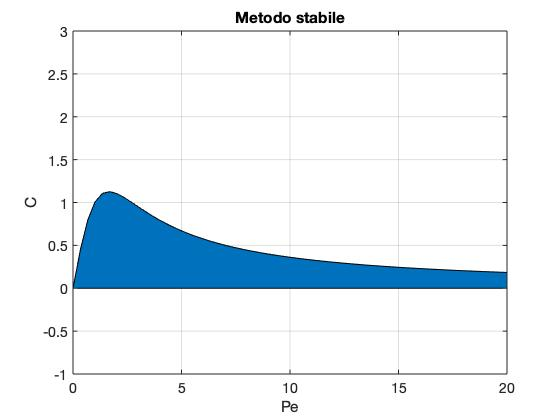
\includegraphics[width=0.95\linewidth]{stabilita1.jpg}
\\

\end{center}


\subsection{}
Per implementare il problema di convezione–diffusione tempo dipendente partiamo dall'equazione discretizzata del problema con la costante di diffusione D=1.
$$\frac{u^{n+1}_j-u^{n}_j}{\Delta t}=-\beta \frac{u^{n}_{j+1}-u^{n}_{j-1}}{2\Delta x}+\frac{u^{n}_{j+1}-2u^{n}_{j}+u^{n}_{j-1}}{\Delta x^{2}}$$
$$\frac{u^{n+1}_j}{\Delta t}=\frac{u^{n}_j}{\Delta t}-\beta \frac{u^{n}_{j+1}-u^{n}_{j-1}}{2\Delta x}+\frac{u^{n}_{j+1}-2u^{n}_{j}+u^{n}_{j-1}}{\Delta x^{2}}$$
$$u^{n+1}_{j}=u^{n}_{j}-\beta\Delta t \frac{u^{n}_{j+1}-u^{n}_{j-1}}{2\Delta x}+\Delta t\frac{u^{n}_{j+1}-2u^{n}_{j}+u^{n}_{j-1}}{\Delta x^{2}}$$
$$u^{n+1}_{j}=u^{n}_{j+1}(\frac{-\beta\Delta t}{2\Delta x}+\frac{\Delta t}{\Delta x^{2}})+u^{n}_{j}(1-\frac{2\Delta t}{\Delta x^{2}})+u^{n}_{j-1}(\frac{\beta\Delta t}{2\Delta x}+\frac{\Delta t}{\Delta x^{2}})$$
Definiamo\newline
$$a1=\frac{-\beta\Delta t}{2\Delta x},\hspace{0.5cm}b1=1-\frac{2\Delta t}{\Delta x^{2}},\hspace{0.5cm}c1=\frac{\beta\Delta t}{2\Delta x}+\frac{\Delta t}{\Delta x^{2}}$$
Ora implementiamo in Matlab il seguente metodo prendendo come costante di convezione $\beta=1$,$\Delta x=1/60$ e $\Delta t=0.8*\Delta x^{2}/2$ e imponendo le condizioni al contorno di Dirichlet in x=0 e x=1 e le condizioni iniziali in modo tale che u(x,t) sia la soluzione esatta.\newline
Con questi valori di D, $\beta,\Delta x,\Delta t$  calcoliamo C e Pe e notiamo che il punto (Pe,C) appartiene alla regione di stabilità definita sopra.\newline 
Rappresentiamo ora nel grafico la soluzione discreta e quella esatta al tempo finale.
\begin{center}
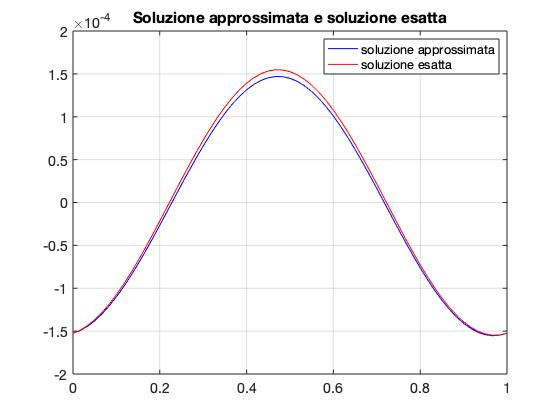
\includegraphics[width=0.95\linewidth]{solesatta.jpg}

\end{center}



\noindent In conclusione possiamo affermare che la soluzione discreta approssima bene la soluzione esatta.\\





\section{Esercizio 2}

\subsection{}
Discretizziamo il problema su una griglia quadrata, in modo da poter considerare uguali gli step $\bigtriangleup x$ e $\bigtriangleup y$. Sia quindi $h = \bigtriangleup x = \bigtriangleup y $.

Manipoliamo il sistema per ricondurci ad una equazione ad un passo:
Inannanzitutto sommiamo le equazioni, ottenendo:
\begin{equation}
\frac{u^{k+1}_{i,j}-u^k_{i,j}}{\bigtriangleup t} = 2 \frac{u^{k+\frac{1}{2}}_{i-1,j} -2u^{k+\frac{1}{2}}_{i,j} + u^{k+\frac{1}{2}}_{i+1,j}}{h^2} + \frac{u^{k}_{i,j-1} -2u^{k}_{i,j} + u^{k}_{i,j+1}}{h^2} + \frac{u^{k+1}_{i,j-1} -2u^{k+1}_{i,j} + u^{k+1}_{i,j+1}}{h^2} + f^{k+\frac{1}{2}}_{i,j}
\end{equation}

Osserviamo che vale l'uguaglianza $u^{k+\frac{1}{2}} = \frac{ u^{k+1}+ u^{k}}{2}$, e sostituiamo i termini $u^{k+\frac{1}{2}}$ in questo modo. Avremo quindi
\begin{equation}
\frac{u^{k+\frac{1}{2}}_{i-1,j} -2u^{k+\frac{1}{2}}_{i,j} + u^{k+\frac{1}{2}}_{i+1,j}}{h^2} = \frac{1}{2} \frac{u^{k+1}_{i-1,j} + u^{k}_{i-1,j} - 2(u^{k+1}_{i,j} + u^{k}_{i,j}) + u^{k+1}_{i+1,j} + u^{k}_{i+1,j}}{h^2}
\end{equation}

Inseriamo questa quantita' in (1), che cosi' diventa

\begin{equation}
\begin{split}
\frac{u^{k+1}_{i,j}-u^k_{i,j}}{\bigtriangleup t} \quad = \quad  \frac{u^{k+1}_{i-1,j} + u^{k}_{i-1,j} - 2(u^{k+1}_{i,j} + u^{k}_{i,j}) + u^{k+1}_{i+1,j} + u^{k}_{i+1,j}}{h^2} +\\ \frac{u^{k}_{i,j-1} -2u^{k}_{i,j} + u^{k}_{i,j+1}}{h^2} + \frac{u^{k+1}_{i,j-1} -2u^{k+1}_{i,j} + u^{k+1}_{i,j+1}}{h^2} + f^{k+\frac{1}{2}}_{i,j}
\end{split}
\end{equation}

\begin{equation}
\begin{split}
\frac{u^{k+1}_{i,j}-u^k_{i,j}}{\bigtriangleup t}  \quad = \quad  \frac{u^{k}_{i-1,j} -2u^{k}_{i,j} + u^{k}_{i+1,j}}{h^2}  +  \frac{u^{k}_{i,j-1} -2u^{k}_{i,j} + u^{k}_{i,j+1}}{h^2}  + \\
\frac{u^{k+1}_{i-1,j} -2u^{k+1}_{i,j} + u^{k+1}_{i+1,j}}{h^2}  +  \frac{u^{k+1}_{i,j-1} -2u^{k+1}_{i,j}  +  u^{k+1}_{i,j+1}}{h^2} + f^{k+\frac{1}{2}}_{i,j}
\end{split}
\end{equation}
Moltiplichiamo (4) per $\bigtriangleup t$ e la riscriviamo come

\begin{equation}
\begin{split}
u^{k+1}_{i,j}  \quad = \quad  u^k_{i,j}+ \quad  \frac{\bigtriangleup t}{h^2} (u^{k}_{i-1,j} -2u^{k}_{i,j} + u^{k}_{i+1,j})  \quad + \quad 
\frac{\bigtriangleup t}{h^2} (u^{k}_{i,j-1} -2u^{k}_{i,j} + u^{k}_{i,j+1})  \quad + \\
\quad + \quad \frac{\bigtriangleup t}{h^2} (u^{k+1}_{i-1,j} -2u^{k+1}_{i,j} + u^{k+1}_{i+1,j}) \quad + \quad \frac{\bigtriangleup t}{h^2} (u^{k+1}_{i,j-1} -2u^{k+1}_{i,j} + u^{k+1}_{i,j+1}) \quad + \quad \bigtriangleup t f^{k+\frac{1}{2}}_{i,j}
\end{split}
\end{equation}

Si tratta quindi di un'equazione a un passo implicita. Vogliamo adesso calcolare l'errore di troncamento: sostituiamo ai termini approssimati $u$ la soluzione esatta, evidenziando gli incrementi al variare degli indici, per poi scriverne lo sviluppo di Taylor. Omettiamo i pedici per non appesantire la notazione, in ogni caso lo sviluppo sara' centrato in $(t_k, x_{ij}, y_{ij})$: passare da $t_k$ a $t_{k+1}$ equivale a un incremento di $\bigtriangleup t$; passare da $u_{i,j}$ a $u_{i+1,j}$ equivale a un incremento di $h$ in $x$ (analogo per $j$, con l'incremento nella direzione $y$).
\begin{equation}
\begin{split}
u(t+ \bigtriangleup t, x, y)  \quad = \quad  u(t, x, y)  \quad + \quad  \frac{\bigtriangleup t}{h^2} \left[u(t, x-h, y) -2u(t,x,y) + u(t, x+h, y)\right]  \quad +\\
+ \quad \frac{\bigtriangleup t}{h^2} \left[u(t, x, y-h) -2u(t,x,y) + u(t, x, y+h)\right]  \quad +\\
+ \quad \frac{\bigtriangleup t}{h^2} \left[u(t+\bigtriangleup t, x-h, y) -2u(t+ \bigtriangleup t,x,y) + u(t+ \bigtriangleup t, x+h, y)\right]  \quad +\\
+ \quad \frac{\bigtriangleup t}{h^2} \left[u(t +\bigtriangleup t, x, y-h) -2u(t+\bigtriangleup t,x,y) + u(t+\bigtriangleup t, x, y+h)\right]  \quad +  \quad \bigtriangleup t f^{k+\frac{1}{2}}_{i,j}
\end{split}
\end{equation}

Consideriamo il trinomio
\begin{center}
	$\frac{\bigtriangleup t}{h^2} (u^{k+1}_{i-1,j} -2u^{k+1}_{i,j} + u^{k+1}_{i+1,j})$
\end{center}
sostituiamo la soluzione esatta nelle $u$, e sviluppiamo ciascun termine fino al IV ordine:

\begin{equation}
\begin{split}
u^{k+1}_{i+1,j} = u(t,x,y) + ((\bigtriangleup t) u_t + h u_x) + (\frac{h^2}{2} u_{xx} + \frac{(\bigtriangleup t)^2}{2} u_{tt} + h (\bigtriangleup t) u_{tx})\\ + (\frac{(\bigtriangleup t)^3}{6} + 3h \frac{(\bigtriangleup t)^2}{2} u_{ttx}  + 3\frac{h^2}{2} (\bigtriangleup t) u_{txx} + \frac{h^3}{6} u_{xxx})\\ + \frac{(\bigtriangleup t)^4}{4!} u_{tttt} + \frac{h^4}{4!} u_{xxxx} - \frac{4 (\bigtriangleup t)^3 h}{6} u_{tttx} + \frac{4 (\bigtriangleup t) h^3}{6} u_{txxx} + \frac{6 (\bigtriangleup t)^2 h^2}{4} u_{ttxx}\\ + O(h^4) + O((\bigtriangleup t)^4) + O((\bigtriangleup t)^3 h) + O((\bigtriangleup t)^2 h^2) + O((\bigtriangleup t) h^3) + O((\bigtriangleup t)^4)
\end{split}
\end{equation}

\begin{equation}
\begin{split}
u^{k+1}_{i,j} = u(t,x,y) + (\bigtriangleup t) u_t + \frac{(\bigtriangleup t)^2}{2} u_{tt} + (\frac{(\bigtriangleup t)^3}{3!}) u_{ttt} + (\frac{(\bigtriangleup t)^4}{4!}) u_{tttt} + O(h^3)\\ + O((\bigtriangleup t)^3) + O((\bigtriangleup t)^2 h^2) + O((\bigtriangleup t)^2 h^2) + O((\bigtriangleup t) h^3) + O((\bigtriangleup t)^4) + O(h^4)
\end{split}
\end{equation}

\begin{equation}
\begin{split}
u^{k+1}_{i-1,j} = u(t,x,y) + ((\bigtriangleup t) u_t - h u_x) + (\frac{h^2}{2} u_{xx} + (\frac{(\bigtriangleup t)^2}{2} u_{tt} - h (\bigtriangleup t) u_{tx}) \\+ (\frac{(\bigtriangleup t)^3}{6} - 3h \frac{(\bigtriangleup t)^2}{2} u_{ttx}  + 3\frac{h^2}{2} (\bigtriangleup t) u_{txx} - \frac{h^3}{6} u_{xxx})\\ + \frac{(\bigtriangleup t)^4}{4!} u_{tttt} + \frac{h^4}{4!} u_{xxxx} - \frac{4 (\bigtriangleup t)^3 h}{6} u_{tttx} - \frac{4 (\bigtriangleup t) h^3}{6} u_{txxx} + \frac{6 (\bigtriangleup t)^2 h^2}{4} u_{ttxx}\\ + O(h^4) + O((\bigtriangleup t)^4) + O((\bigtriangleup t)^3 h) + O((\bigtriangleup t)^2 h^2) + O((\bigtriangleup t) h^3) + O((\bigtriangleup t)^4)
\end{split}
\end{equation}

sommando i tre sviluppi:
\begin{equation}
\bigtriangleup t\frac{(u^{k+1}_{i-1,j} -2u^{k+1}_{i,j} + u^{k+1}_{i+1,j})}{h^2}  = (\bigtriangleup t)u_{xx} + 3(\bigtriangleup t)^2 u_{txx} + O(h^3) + O((\bigtriangleup t)^3) + ...
\end{equation}
quindi l'errore di troncamento per questo trinomio vale:
\begin{equation}
\tau^{k+1}_{dx} = \frac{(u^{k+1}_{i-1,j} -2u^{k+1}_{i,j} + u^{k+1}_{i+1,j})}{h^2}  - u_{xx} = 3(\bigtriangleup t) u_{txx} + O(
h^3 \bigtriangleup t) + O((\bigtriangleup t)^2) + ...
\end{equation}

in modo analogo si possono sviluppare tutte le componenti di (6), e sottrarre l'equazione esatta per ricavare l'errore di troncamento dell'equazione (5), che quindi vale
\begin{equation}
\tau = c_1 (\bigtriangleup t) + c_2 h^2 + O((\bigtriangleup t)^2) + O(h^3) + ...
\end{equation}
con $c_1, c_2 \in \textbf{R}$.\\
In realta', trattandosi di una semidiscretizzazione in tempo, per calcolare l'ordine in tempo possiamo considerare la parte spaziale come continua anziche' discreta, guadagnando cosi' un ordine in tempo. Dunque il metodo dovrebbe avere ordine teorico 2 sia in spazio che in tempo.
Inoltre il metodo e' consistente in quanto, per
\begin{center}
	$\bigtriangleup t \rightarrow 0$\\
	$h \rightarrow 0$
\end{center}
si ha
\begin{center}
	$\tau (\bigtriangleup t, h) \rightarrow 0$
\end{center}

\subsection{}
Consideriamo ora le equazioni di partenza. Definiamo $\mu := \frac{\bigtriangleup t}{h^2}$. Separiamo le quantita' note da quelle incognite, portando queste ultime a sinistra dell'uguaglianza, ottenendo cosi':

\begin{equation}
\begin{cases}
-\mu u^{k+\frac{1}{2}}_{i-1,j} + (1+2\mu)u^{k+\frac{1}{2}}_{i,j} -\mu u^{k+\frac{1}{2}}_{i+1,j} = \mu u^{k}_{i,j-1} + (1-2\mu) u^{k}_{i,j} + \mu u^{k}_{i,j+1} + \frac{\bigtriangleup t}{2} f^{k+\frac{1}{2}}_{i,j}\\ 

-\mu u^{k+1}_{i,j-1} + (1+2\mu)u^{k+1}_{i,j} -\mu u^{k+1}_{i,j+1} = \mu u^{k+\frac{1}{2}}_{i-1,j} + (1-2\mu) u^{k+\frac{1}{2}}_{i,j} + \mu u^{k}_{i,j} + \frac{\bigtriangleup t}{2} f^{k+\frac{1}{2}}_{i,j}

\end{cases}
\end{equation}

Abbiamo ritenuto piu' opportuno separare le equazioni in piu' sistemi, nel seguente modo:

Discretizziamo entrambi gli assi x,y con $n$ nodi ciascuno, ottenendo una griglia quadrata con $n^2$ punti. Avremo quindi $n-2$ punti interni per lato.
Sia A la matrice $(n-2) \times (n-2)$ di iterazione del lato sinistro
\begin{center}
	$
	A = \begin{bmatrix}
	1+2\mu & -\mu & 0 & 0 & \cdots & 0 \\
	-\mu & 1+2\mu & -\mu & 0 & \cdots & 0\\
	0 & -\mu & 1+2\mu & -\mu & \cdots & 0\\
	\vdots &  & \ddots & \ddots  & \ddots\\
	\\
	& &  &  &   & -\mu\\
	0 &  &  \cdots & 0  & -\mu & 1+2\mu\\ 
	\end{bmatrix}
	$
\end{center}
Per la prima equazione:\\
Fissiamo l'indice di colonna $j = 1$ e iteriamo su $i$. Al variare di $i = 1,...,n-2$  otteniamo il sistema
\begin{equation}
A {\begin{pmatrix}
	u_{1,1}\\
	u_{2,1}\\
	\vdots\\
	u_{n-2,1}
	\end{pmatrix}}^{k+\frac{1}{2}} = 
\begin{cases}
(1-2\mu)u^k_{1,1} + \mu u^k_{1,2} + \frac{\bigtriangleup t}{2} f^{k+\frac{1}{2}}_{1,1} + \mu \color{blue}{(u^k_{1,0} + u^{k+\frac{1}{2}}_{0,1})}\\
(1-2\mu)u^k_{2,1} + \mu u^k_{2,2} + \frac{\bigtriangleup t}{2} f^{k+\frac{1}{2}}_{2,1} + \mu \color{blue}{(u^k_{2,0})}\\
\quad \vdots\\
(1-2\mu)u^k_{n-3,1} + \mu u^k_{n-3,2} + \frac{\bigtriangleup t}{2} f^{k+\frac{1}{2}}_{n-3,1} + \mu \color{blue}{(u^k_{n-3,0})}\\
(1-2\mu)u^k_{n-2,1} + \mu u^k_{n-2,2} + \frac{\bigtriangleup t}{2} f^{k+\frac{1}{2}}_{n-2,1} + \mu \color{blue}{(u^k_{n-2,0} + u^{k+\frac{1}{2}}_{n-1,1})}\\
\end{cases}
\end{equation}
dove le quantita' in blu sono date dalle condizioni al bordo.
Analogamente, per $j = 2,...,n-3 $ avremo i sistemi:
\begin{equation}
A {\begin{pmatrix}
	u_{1,j}\\
	u_{2,j}\\
	\vdots\\
	u_{n-2,j}
	\end{pmatrix}}^{k+\frac{1}{2}} = 
\begin{cases}
\mu u^k_{1,j-1} + (1-2\mu)u^k_{1,j} + \mu u^k_{1,j+1} + \frac{\bigtriangleup t}{2}f^{k+\frac{1}{2}}_{1,j} + \mu \color{blue}{(u^{k+\frac{1}{2}}_{0,j})}\\
\mu u^k_{2,j-1} + (1-2\mu)u^k_{2,j} + \mu u^k_{2,j+1} + \frac{\bigtriangleup t}{2}f^{k+\frac{1}{2}}_{2,j}\\
\quad \vdots\\
\mu u^k_{n-3,j-1} + (1-2\mu)u^k_{n-3,j} + \mu u^k_{n-3,j+1} + \frac{\bigtriangleup t}{2}f^{k+\frac{1}{2}}_{n-3,j}\\
\mu u^k_{n-2,j-1} + (1-2\mu)u^k_{n-2,j} + \mu u^k_{n-2,j+1} + \frac{\bigtriangleup t}{2}f^{k+\frac{1}{2}}_{n-2,j} + \mu \color{blue}{(u^{k+\frac{1}{2}}_{n-1,j})}\\
\end{cases}
\end{equation}
il caso $j = n-2$ e' analogo a (14).\\
Chiamiamo $bcs$ il vettore delle condizioni al bordo, e $b$ il restanto lato destro delle equazioni.
Ciascun sistema e' quindi della forma
\begin{center}
	$Au^{k+\frac{1}{2}}_j = b + bcs$
\end{center}
ed essendo A tridiagonale possiamo risolverli con l'algoritmo di Thomas. Ciascuna soluzione corrisponde ad una colonna della matrice  $u^{k+\frac{1}{2}}$, di dimensioni $(n-2) \times (n-2)$, che corrisponde alla soluzione approssimata sulla griglia interna al tempo $k+\frac{1}{2}$.\\

Essendo ora la matrice $u^{k+\frac{1}{2}}$ nota, la inseriamo nella seconda equazione per calcolare $u^{k+1}$.
Questa volta fissiamo l'indice di riga $i$ e facciamo variare l'indice di colonna $j = 2,...,n-2$.
Le equazioni che si ottengono sono pressoche' identiche a quelle precedenti, con $u^{k+\frac{1}{2}}$ sul lato destro e $u^{k+1}$ sul lato sinistro, e indici $i$ e $j$ scambiati.\\
Per ciascuna equazione dobbiamo quindi risolvere $n-2$ sistemi lineari. In totale abbiamo quindi $2(n-2)$ sistemi. Ogni sistema viene risolto dall'algoritmo di Thomas in $O(n-2)$ operazioni. Il costo computazionale totale dovrebbe quindi essere $O((n-2)^2)$.

\subsection{}
Innanzitutto ricaviamo le funzioni che descrivono le condizioni al bordo imponendo i valori di x e y a seconda dei casi:\\
$ gN = u(x,1,t) = \frac{1}{\sqrt{1+4t}} e^{(-\frac{x^2+1}{1+4t})}\\
gS = u(x,0,t) = \frac{1}{\sqrt{1+4t}} e^{(-\frac{x^2}{1+4t})}\\
gO = u(0,y,t) = \frac{1}{\sqrt{1+4t}} e^{(-\frac{y^2}{1+4t})}\\
gE = u(1,y,t) = \frac{1}{\sqrt{1+4t}} e^{(-\frac{y^2+1}{1+4t})}
$\\

e il termine sorgente:\\
$f(x,y,t) = \frac{2}{(1+4t)^{\frac{3}{2}}} e^{(-\frac{x^2+y^2}{1+4t})}$\\

Facciamo notare che nel codice Matlab le funzioni $gN$ e $gS$ sono scambiate per tenere conto del fatto che la rappresentazione matriciale della griglia non corrisponde alla griglia teorica nel piano cartesiano.\\

Purtroppo non siamo state in grado di verificare sperimentalmente l'ordine del metodo. Il programma infatti approssima correttamente la soluzione esatta (come si vede dai grafici prodotti e dal fatto che l'errore si mantiene sempre < $10^{-2}$), ma aumentando il numero di nodi e/o raffinando il tempo l'errore aumenta. Cio' si discosta dalle aspettative. Possiamo ipotizzare si tratti di un errore nel codice o di errori di floating, ma non siamo in grado di dare una motivazione precisa.

Alleghiamo comunque i grafici della soluzione approssimata e dell'errore che illustrano quanto detto:
\begin{figure}[H]
	\centering
	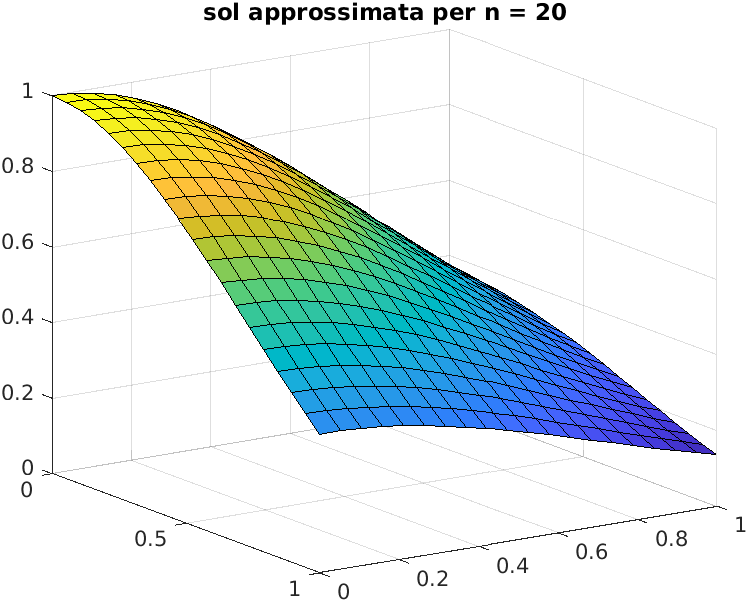
\includegraphics[totalheight=8cm]{grafico.png}
	\caption{Soluzione approssimata}
	\label{fig:verticalcell}
\end{figure}

\begin{figure}[H]
	\centering
	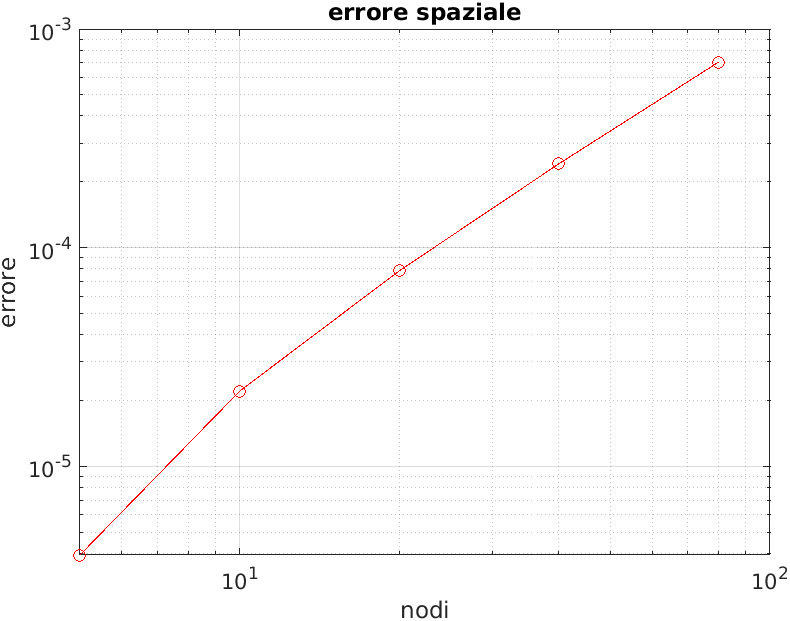
\includegraphics[totalheight=8cm]{errore_es2.png}
	\caption{Andamento dell'errore}
	\label{fig:verticalcell}
\end{figure}


\end{document}